\chapter{Introduction}
\label{ch:introduction}

\newcommand{\IncludeGraphicsOrPlaceholder}[2][]{%
  \IfFileExists{#2}{%
    \includegraphics[#1]{#2}%
  }{%
    \fbox{%
      \parbox[c][0.22\textheight][c]{0.9\linewidth}{%
        \centering Missing figure file\\\texttt{\detokenize{#2}}%
      }%
    }%
  }%
}

A structurally correct sequence of notes is only the foundation of a musical performance. When performers receive a composed score, they do not merely execute a rigid sequence of instructions. They interpret the piece and bring it to expressiveness. A central dimension of this interpretation is musical dynamics. This involves the deliberate shaping of loudness over individual notes, phrases, and larger formal units. Dynamics conveys emotional nuance. It balances voices inside a texture and shapes the direction of a phrase. It is often the clearest signal that separates a convincing human performance from a flat mechanical rendering.

Msical performance is commonly represented in two complementary symbolic forms. The first is MIDI, where note events are paired with note-level control parameters such as velocity. MIDI velocity records the action intensity at note onset. It is precise, machine-readable, and directly editable, mostly comes from the sensor physical measures. The second is the music score, where dynamics is represented by human-readable markings such as \textit{pp}, \textit{p}, \textit{mf}, \textit{f}, \textit{ff}. These markings are relative, context-dependent, and less precise as physical measurements, but they communicate musical intent on a musically meaningful metrical grid. 

Automatic Music Transcription (AMT) aims to bridge human performance audio and symbolic music representations, including MIDI and scores. Driven by deep learning and large aligned datasets \cite{hawthorne2019maestro}, recent AMT systems can transcribe note events with high accuracy. Yet this progress remains asymmetric \cite{amt2019ov}. The field is proficient at recovering what notes are played and when they occur. It is much less mature at recovering how loud those notes are played in terms of the dynamics shaping and other expressive dimensions, as depicted in Figure~\ref{fig:intro_expressive_amt}

This thesis posits that dynamics is a foundational component of expressive AMT. While music expression is multifaceted, dynamics represents the most perceptually salient and practically essential dimension. Unlike a standard transcription that yields flat intensities, a dynamics-aware approach enables expressive rendering and high-quality symbolic corpora curation. By focusing on the robust recovery of score dynamics and MIDI velocity, this work provides a critical layer of musical information.

\begin{figure}[h!]
  \centering
  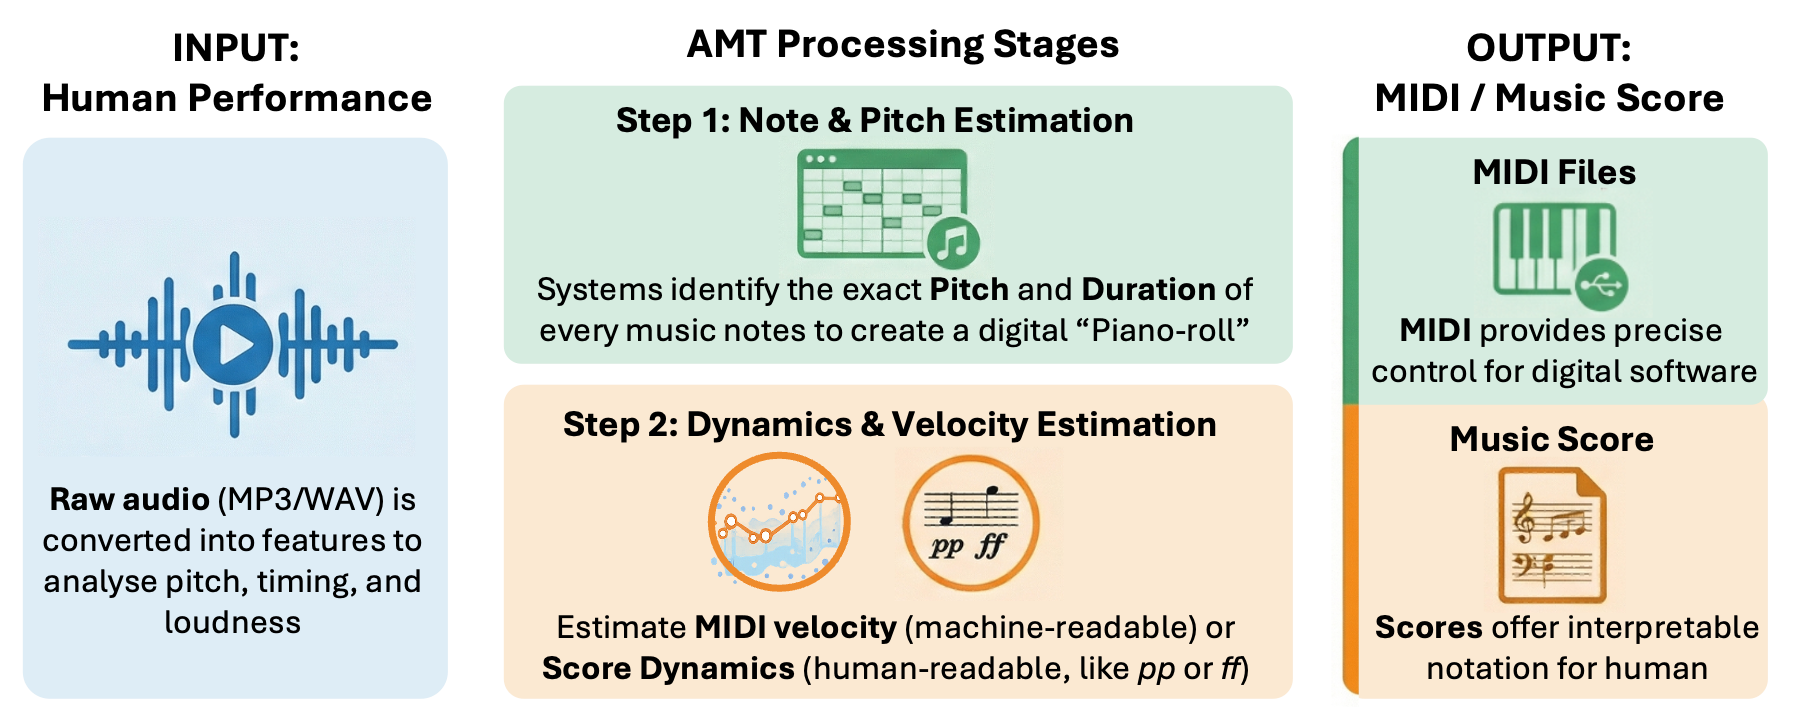
\includegraphics[width=\linewidth]{Chapter_1/figures/AMT.png}
  \caption{The general architecture of an AMT system, illustrating the transformation of raw acoustic audio into foundational note events and expressive dynamic information. The pipeline results are MIDI data and musical scores.}
  \label{fig:intro_expressive_amt}
\end{figure}

\section{Motivation}
\label{sec:motivation}

Transcribing correct pitches and timing is only the foundational step of AMT. Incorporating dynamics into transcription results significantly enhances their capacity to carry expressive intent, taking the form of MIDI velocity or score dynamics. This is not only a technical improvement. Transitioning toward such expressive AMT unlocks significant practical benefits, as outlined below:

\paragraph{MIDI production and expressive rendering.} 
MIDI is the dominant representation in digital music production, supporting efficient editing and flexible rendering. Yet, much software-generated MIDI is created via step input and quantisation, leaving expressive parameters at a lifeless, default constant. Among these, MIDI velocity is one of the most accessible control variables for shaping note intensity and expressive contour \cite{dan2006psy,palamara2020dynamic}. Creators often want to preserve their composed notes and timing. To inject human-like expression, they simply need to adjust velocity values. Still, manual editing is time-consuming and delicate. Developing automated methods for velocity completion becomes an essential step for realistic rendering.

\paragraph{Music education and performance feedback.} 
Score dynamics is also a core pedagogical dimension. In automatic piano performance assessment, dynamics is routinely treated alongside pitch, timing, and rhythm as one of the salient components of performance quality and feedback \cite{kim2022piano}. More recent work on query-based music coaching likewise emphasises that useful educational feedback needs interpretable information about expressive shaping, not only note correctness \cite{zhang2025llaqo,park2025dynvisual}. In many educational scenarios, a reference score is already available together with a student performance audio. This makes score-informed dynamics estimation especially attractive, because the symbolic prior can stabilise the prediction while keeping the feedback musically meaningful.

\paragraph{Expressive data curation by enhancing existing archives.}
A third motivation comes from data curation. Many large-scale music archives provide aligned audio and symbolic content (MIDI sequences or digital scores). However, expressive labels are consistently missing. Velocities are often flattened to a default value, and score dynamic markings are absent or unreliable, limiting the utility of these corpora for downstream applications. Furthermore, a deep semantic gap exists between physical machine measurements (MIDI velocity) and subjective human cognition (score dynamics). Bridging this gap and recovering these missing dimensions is imperative to upgrade static archives into richly expressive datasets.

By contrast, recollecting new datasets from scratch is a costly process constrained by audio-to-score synchronisation challenges, required musical expertise, and copyright restrictions \cite{li2019urmp,foscarin2020asap,morsi2022bottlenecks}. Therefore, this thesis treats \emph{label recovery} as a scalable, principled strategy. By retroactively estimating missing dynamics on existing corpora, we entirely bypass acquisition bottlenecks and annotation ambiguities, unlocking a vast, previously untapped resource for data-driven music research.

\section{Dynamics as a Target in Expressive AMT}
\label{sec:intro:why_dynamics}

Expressive AMT extends beyond recovering mere pitch and onset/offset boundaries to capture the full aspects of a human performance. A comprehensive expressive transcription can be conceptually divided into three primary layers:
\begin{itemize}
\item \textbf{Timing Layer:} Captures the temporal elasticity of a performance, encompassing macro-level tempo variations, beat tracking, inter-onset intervals (IOI), and micro-level articulation.
\item \textbf{Dynamic Layer:} Represents the intensity and energy of the musical execution, bridging physical machine measurements (e.g., MIDI velocity) with semantic cognitive notations (e.g., score dynamic markings).
\item \textbf{Control Layer:} Includes instrument-specific techniques and acoustic modifiers, such as sustain pedaling, vibrato, reverberation, and amplifier configurations.
\end{itemize}
While all three layers are essential for a complete computational understanding of performance, this thesis isolates the \textbf{Dynamic Layer} as its primary expressive target. This focus does not imply that timing or control parameters are secondary. Rather, dynamics is chosen to move AMT beyond note content for three reasons:

\paragraph{Perceptual salience.}
Dynamics is one of the most immediately audible dimensions of expressive performance. Listeners often perceive phrase direction, accent, and balance through intensity change before they perceive subtler aspects such as pedaling or micro-timing. A transcription that omits dynamics therefore omits a central part of musical meaning.

\paragraph{Symbolic editability.}
Compared to complex continuous controls like overdrive (electric guitar) or pedaling (piano), dynamics offers an exceptionally tractable and editable symbolic representation. MIDI velocity serves as a universal, loudness control parameter for all instrumentsin digital audio workstations (DAWs), while score dynamics provide a standard notational device for composition, pedagogy, and performance analysis. This dual nature makes dynamics a robust bridge between low-level MIR outputs and high-level musical practice.

\paragraph{Recoverability across realistic data conditions.}
Many expressive targets require fine-grained, instrument-specific mechanisms, particularly within the Control Layer. They are entirely absent or poorly labeled in existing large-scale music datasets. Dynamics, while challenging to estimate accurately, remains highly recoverable across various practical paradigms. It therefore provides a scalable entry point for advancing expressive AMT without being bottlenecked by instrument-specific data scarcity.

\section{Two Complementary Forms of Dynamics}
\label{sec:intro:two_forms}
Having established dynamics as our primary expressive target, we clarify its two complementary symbolic forms within this thesis, as summerized in Table \ref{tab:intro_two_forms}.

\begin{table}[b]
\centering
\caption{Two complementary forms of dynamics that recur throughout this thesis.}
\label{tab:intro_two_forms}
\fontsize{11pt}{13pt}\selectfont
\setlength{\tabcolsep}{4pt}
\renewcommand{\arraystretch}{1.2}
\begin{tabularx}{\textwidth}{llll}
\toprule
\textbf{Representation} & \textbf{Nature} & \textbf{Temporal Anchor} & \textbf{Primary Carrier} \\
\midrule
MIDI velocity & \makecell[l]{Physical\\measurement} & \makecell[l]{Note-level: isolated value\\at each note} & \makecell[l]{DAWs, electronic\\instruments (synthesisers)} \\
Score dynamics & \makecell[l]{Subjective\\intention} & \makecell[l]{Metrical-level: shared value\\in a beat/phrase} & \makecell[l]{Digital sheet music,\\human performers} \\
\bottomrule
\end{tabularx}
\end{table}

\paragraph{MIDI velocity.}
Originating from the physical sensors of electronic keyboards and pianos, MIDI velocity is a machine-centric measurement of physical intensity. To say it operates as a "note-level" parameter means that every music note from a discrete key strike is assigned an independent, static integer representing its initial strike force. This strict per-note measurement dictates that velocity functions as a discrete loudness control parameter. It is highly granular and absolute within its own scale, yet the resulting loudness highly depends on the acoustic environment and the specific instrument being played. Because MIDI velocity is necessary for MIDI-to-audio playback in DAWs and synthesizers, a common default is set to 64 when it is missing.

\paragraph{Score dynamics.}
Score dynamics represents the subjective cognitive intention of the composer or performer. Instead of attaching to isolated notes, markings like \textit{p} or \textit{crescendo} are conceptually anchored to the underlying metrical structure, acting as shared values across a specific beat or an entire phrase. This segment-level instruction provides a holistic perception of intensity while leaving room for free human interpretation. Because it is structurally aware and musically meaningful, score dynamics is the ideal target for pedagogical feedback and score analysis. In symbolic environments, the default assumption is often that missing score dynamics should be filled with \textit{mf} (mezzo-forte), which is the neutral middle ground of human perceptual loudness. 

\section{Research Gap and Thesis Stance}
\label{sec:intro:gap_stance}

This section point to a narrower and more practical research gap than the general claim that AMT still lacks expressiveness. A recurring paradox in music research is that while structural data (pitch and timing) is increasingly abundant, expressive data remains systematically impoverished. A MIDI file may contain correct note sequences while leaving all velocities ar a default constant. A performance corpus may preserve audio and aligned scores but only sparse, unreliable, or absent dynamic markings. The common is therefore how to recover a missing expressive label layer from data that are already partly specified.

\paragraph{The ontological gap: dynamics must be inferred across representations.}
This is not a simple label-conversion problem. Audio loudness an acoustic and perceptual phenomenon. MIDI velocity is a machine-centric, physical parameter. Score dynamics is a cognitive, context-dependent notation of musical intention. These three forms are related but encodes different concepts. A method that translates one to another must bridge the fundamental gap between objective physical measurement and subjective human cognition.

\paragraph{The ambiguity of ground truth: dynamics is more fragile than notes.}
For note transcription, pitch and onset often remain learnable under moderate changes in instrument, room, or recording conditions. Dynamics ground truth is less stable. Small changes in instruments (timbre), microphone placement, editorial convention, or synthesis setup can alter the apparent relation between sound, MIDI velocity, and score dynamics notation. For non-piano settings, the difficulty becomes sharper because the bottleneck is not ordinary domain shift but missing measurement itself: reliable MIDI velocity labels are rarely available, and in some cases even the ground truth is instrument-dependent.

\paragraph{Fragmented supervision regimes.}
The MIR community lacks a singular, omnipotent dataset that pairs audio with both cognitive score annotations and physical velocity labels. Supervision is deeply fragmented: some corpora provide aligned scores without performance control, while others provide precise velocity data but no human-readable score. A robust thesis on expressive dynamics cannot rely on an idealized, fully supervised data regime. It must systematically address these disjointed data environments.

\paragraph{Thesis stance: label recovery under structural preservation.}
For these reasons, this thesis adopts a unified \emph{label-recovery} perspective. It does not treat the problem as music generation, full expressive rendering, or style transfer. Instead, it asks a narrower, more pragmatic question: when pitch, onset, and often alignment are already trusted, how can the missing dynamics labels be recovered without rewriting the note content or trusted timing? The ultimate goal is to recover labels that remain musically interpretable and directly usable—whether as note-level MIDI velocity for production workflows, or as beat-synchronous score dynamics for pedagogy and analysis.

\section{Unified Thesis Question and Three Core Scenarios}
\label{sec:intro:question}

The thesis is driven by the following question:

\begin{quote}
\textbf{How can musically interpretable dynamics labels be recovered from incomplete, weakly expressive, or weakly supervised music data without rewriting note content or note timing?}
\end{quote}

That question is studied under three core scenarios.

\begin{table}[t]
\centering
\caption{The three core supervision scenarios studied in this thesis.}
\label{tab:intro_scenarios}
\small
\setlength{\tabcolsep}{4pt}
\renewcommand{\arraystretch}{1.15}
\begin{tabularx}{\textwidth}{l X X X X}
\toprule
\textbf{Scenario} & \textbf{Available data} & \textbf{Missing label} & \textbf{Target output} & \textbf{Position} \\
\midrule
S1 & MIDI note sequence & note-level expressive intensity & MIDI velocity completion & Chapter~3 \\
S2 & performance audio + aligned MIDI (score) & reliable note-level expressive intensity & score-informed MIDI velocity refinement & Chapter~4 \\
S3 & performance audio only & human-readable score-facing dynamics and metrical coordinates & beat-synchronous dynamic levels, change points, beats, downbeats & Chapter~5 \\
\bottomrule
\end{tabularx}
\end{table}

\begin{enumerate}
    \item \textbf{Scenario S1: symbolic-only MIDI velocity completion.} The note content and timing are already available in MIDI form, but the velocity is missing or flattened. The goal is to complete note-level velocity from symbolic structure alone.

    \item \textbf{Scenario S2: audio-plus-score velocity refinement.} A performance recording is available together with an aligned score. While the AMT audio-only velocity estimation serves as a plausible but optimizable baseline, the goal is to refine this velocity by using the score as a structural prior.

    \item \textbf{Scenario S3: audio-only score-dynamics recovery.} Only the performance audio is available, and the goal is not raw note-level velocity but beat-synchronous score dynamics. The system must therefore recover dynamic levels together with the metrical structure needed to place them on a symbolic score.
\end{enumerate}

These three scenarios are intentionally ordered from the most controlled setting to the most open one. Scenario S1 isolates dynamics recovery by assuming symbolic notes are already available. Scenario S2 adds real audio context while keeping structural support from a score. Scenario S3 removes that support, moving to a more ambiguous, human-readable target. While these three form the core empirical arc, the thesis will also present a brief exploratory extension (Chapter 6) to investigate whether this velocity learning framework can generalize beyond the piano.

\section{Aim, Scope, and Assumptions}
\label{sec:intro:scope}

The aim of this thesis is to develop stand-alone but conceptually linked methods for recovering dynamics-related labels from real music data. The recovered labels include note-level MIDI velocity, beat-synchronous dynamic levels, change points, beats, and downbeats. The intended outcome is not only stronger AMT-style prediction, but also more expressive and more editable symbolic music for downstream use.

The main scope and assumptions are as follows.

\begin{itemize}
    \item \textbf{Primary empirical focus.} The main experimental focus is piano. This is because reliable note-level velocity ground truth remains concentrated on instrumented pianos particularly by the Yamaha Disklavier systems \cite{hawthorne2019maestro}.

    \item \textbf{Preservation of note content and timing.} The thesis does not aim to rewrite the note sequence. Dynamics is treated as a refinement or annotation layer on top of fixed note events.

    \item \textbf{Two complementary outputs.} The thesis studies both note-level MIDI velocity and beat-synchronous score dynamics. It does not force all expressive information into a single representation.

    \item \textbf{Out-of-scope factors.} The thesis does not attempt full modelling of articulation, pedal, timbre, or micro-timing, except when these factors provide indirect context for dynamics recovery.

    \item \textbf{Beyond piano.} Extending velocity estimation beyond piano is recognised as an important direction because piano-centric datasets create a real bias in expressive AMT. However, large-scale non-piano score-dynamics transcription with human labels remains outside the present thesis scope.
\end{itemize}

\section{Main Contributions}
\label{sec:intro:contrib}

The main contributions of this thesis are as follows.

\begin{itemize}
    \item \textbf{A thesis-level formulation of dynamics-oriented label recovery.} The dissertation argues that dynamics should be treated as a first-class target in expressive AMT and organises the problem around heterogeneous supervision regimes rather than one ideal dataset.

    \item \textbf{A symbolic-only method for note-level velocity completion.} Chapter~3 reformulates MIDI velocity completion as an image-colorisation problem on sparse piano-roll representations. It introduces a U-Net with window attention and a sparsity-aware loss, and shows gains in both objective metrics and listening tests \cite{he2025filling}.

    \item \textbf{A modular score-informed correction strategy for AMT velocity estimation.} Chapter~4 introduces a lightweight Transformer correction module that refines AMT-estimated velocity using an aligned score. The design goal is portability across existing AMT backbones rather than a fully bespoke score-informed system.

    \item \textbf{An audio-only framework for beat-synchronous score-dynamics recovery.} Chapter~5 proposes a compact multi-task multi-scale network that jointly estimates dynamic levels, change points, beats, and downbeats. It combines a perceptually motivated Bark-scale specific loudness front-end with task-aware decoding through MMoE \cite{he2026dynest,ma2018mmoe}.

    \item \textbf{An exploratory beyond-piano study based on proxy supervision.} Chapter~6 investigates cross-instrument MIDI velocity estimation when true labels are scarce. It employs a differentiable proxy for black-box synthesizers as part of the supervision signal. This contribution tests a route beyond the piano domain.
\end{itemize}


\begin{figure}[h]
  \centering
  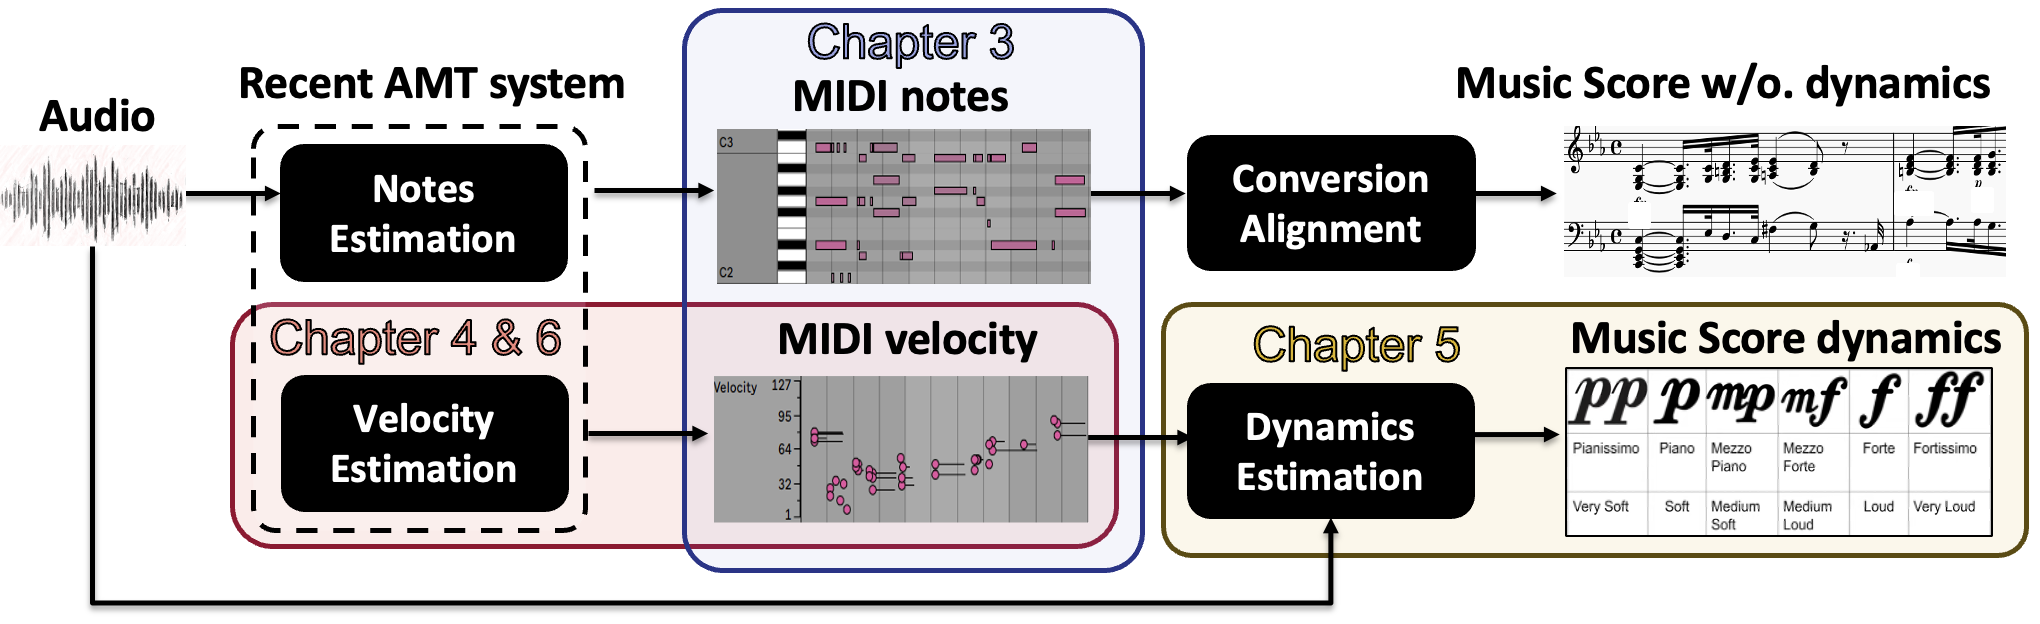
\includegraphics[width=\linewidth]{Chapter_1/figures/Overview.jpg}
  \caption{Shared problem space of the thesis. The dissertation studies dynamics across three linked but non-identical representations: acoustic evidence in audio, note-level performance control in MIDI velocity, and score-facing symbolic intention in notated dynamics.}
  \label{fig:intro_overview}
\end{figure}


\section{Thesis Organisation}
\label{sec:intro:organisation}

Referring Figure~\ref{fig:intro_overview}, the core methodological chapters (Chapters 3--5) preserve the technical contributions of their respective peer-reviewed publications, while expanding the motivation, task-specific related work, and overarching discussion to form a unified narrative. The remainder of the thesis is organised as follows:

\textbf{Chapter~2} establishes the shared conceptual system of the dissertation. It defines what dynamics means across audio, MIDI, and score, and reviewing the AMT models, datasets and evaluation strategies.

\textbf{Chapter~3} addresses Scenario~S1. It formulates symbolic-only MIDI velocity completion as an image-colorisation problem on sparse piano-rolls. Supported by listening tests, it demonstrates that restoring note-level dynamics alone is enough to transform a mechanical MIDI sequence into an expressive, human-like performance, all while keeping the original note content and timing strictly fixed.

\textbf{Chapter~4} addresses Scenario~S2. It introduces a lightweight, portable Transformer correction module that refines AMT-estimated velocity from performance audio using an aligned score as a structural prior. It shows that this approach has better generalisation under dataset shift than AMT baseline, and robustness to audio-to-score misalignment.

\textbf{Chapter~5} addresses Scenario~S3. It proposes an audio-only framework using a multi-task multi-scale network to jointly estimate score dynamic markings and metrical structure, which is the temporal anchor needed to place them into music score.

\textbf{Chapter~6} extends the note-level velocity thread beyond piano. It studies cross-instrument MIDI velocity estimation with proxy supervision. It confronts the dataset bias exposed by earlier chapters by investigating cross-instrument MIDI velocity estimation with proxy supervision, probing the frontier where direct velocity labels disappear.

\textbf{Chapter~7} revisits the unified thesis question, concludes the findings across the four studies, states the limitations clearly, and outlines future directions for expressive AMT.